\part{Tutorial}

\chap{Ihr erstes Roboter-Projekt}\label{ch.intro}

\sect{Thymio kennen lernen}

\Cref{fig.front} zeigt den Roboter Thymio von vorne und von oben. Oben sieht man einen runden Knopf in der Mitte (\textcolor{blue}{A}) und die vier Richtungsknöpfe (\textcolor{blue}{B}). Hinter den Knöpfen wird der Ladezustand der Batterie in grün (\textcolor{blue}{C}) angezeigt. Dahinter sieht man die zwei oberen Lichter (\textcolor{blue}{D}), die auf rot eingestellt sind. Der Roboter hat unten weitere solche Lichter (siehe \Cref{fig.bottom}). Die schmalen schwarzen Rechtecke (\textcolor{blue}{E}) vorne sind Sensoren, die Sie im \cref{ch.pet} kennenlernen werden. 

\begin{figure}[h]
\begin{center}
\gr{front}{.8}
\caption{Thymio Roboter von vorne oben}\label{fig.front}
\end{center}
\end{figure}

\sect{Den Roboter verbinden und VPL starten}

Verbinden Sie Ihren Thymio Roboter mit dem USB Kabel mit dem Computer. Der
Roboter spielt eine kleine Tonabfolge ab und die Oberfläche leuchtet grün. Sollte der Roboter ausgeschaltet sein oder bei der Verbindung sich nicht einschalten, schalten sie ihn ein, indem sie während fünf Sekunden
den mittleren Knopf berühren. Starten sie nun VPL indem sie das VPL-Icon \blksm{thymiovpl} auf ihrem Computer mit Doppelklick anwählen.

\importantbox[Kleine Bilder]{Wenn ein kleines Bild im Text erscheint, wird eine grosse Version davon am Rand dargestellt.}

Möglicherweise verbindet sich VPL automatisch mit ihrem Roboter. Falls dies nicht der Fall sein sollte, wird das Bild wie in \cref{fig.connect} angezeigt. Wählen Sie das Kästchen \bu{Serie} an, klicken Sie auf \bu{Thymio-II Robot ...} darunter, wählen sie die Sprache und klicken sie auf \bu{Verbinden}. Abhängig von der Konfiguration ihres Computers und des Betriebssystems, das sie einsetzen, kann es sein, dass die Einträge im Fenster und die folgenden Daten des Thymio etwas anders ausschauen, als in der Abbildung angezeigt.

\trickbox{Es ist auch möglich VPL aus dem Aseba Studio (textbasierte Programmierumgebung) heraus zu öffnen. Das VPL Plug-in befindet sich unten links im Fenster unter \textit{Tool}.} 

\begin{figure} 
\begin{center}
\gr{connect}{.4}
\caption{Thymio mittels USB-Kabel verbinden}\label{fig.connect}
\end{center}
\end{figure}

\sect{Wireless Thymio}

Es gibt eine Thymio-Version, die der Fähigkeit zur drahtlosen Kommunikation besitzt. Diese müssen nicht via Kabel verbunden werden. Der Wireless-Roboter wird mit einem kleinen Objekt ausgeliefert, dem sogenannten \emph{Dongle}:

\gr{dongle}{.4}

Stecken Sie den Dongle in einen USB-Steckplatz Ihres Computers, schalten Sie den Roboter ein und starten Sie VPL, wie weiter oben beschrieben. Wenn Sie das Verbindungsfenster sehen (Abbildung \ref{fig.connect}) wählen Sie die Zeile mit der Bezeichnung \bu{Thymio-II Wireless (COMnn)}.

\importantbox{Sie benötigen immer noch ein USB-Kabel um den Roboter aufzuladen (Abbildung~\ref{fig.back}).}

\sect{Bedienungsoberfläche von VPL}

Die Bedienungsoberfläche von VPL wird unten angezeigt. Diese ist in sechs
Bereiche aufgeteilt:
\begin{enumerate}[noitemsep,nosep]
\item Oben hat sie eine Symbolleiste mit Symbolen, um Programme zu öffnen, zu speichern, auszuführen, etc.
\item Unterhalb der Symbolleiste befindet sich der Bereich, in dem man Programme für den Roboter erstellt.
\item  In einem Nachrichten-Bereich wird angezeigt, ob das Programm funktioniert oder es werden Fehlermeldungen angezeigt.
\item Links eine Spalte mit den Ereignisblöcken.
\item Weiter rechts eine Spalte mit den Aktionsblöcken zur Konstruktion des Programms.
\item Auf der rechten Seite der Code, wie das Programm in die textbasierte Sprache von Aseba übersetzt wird.
\end{enumerate}

\plainfloat
\begin{figure}[h]
\gr{gui}{1}
\caption{Die Bedienungsoberfläche von VPL}\label{fig.vplgui}
\end{figure}
\framedfloat

\newpage

\informationbox{Weiterführende Informationen}{ Wenn Sie mit VPL ein Programm erstellen, wird eine Übersetzung in die textbasierte Programmiersprache AESL vorgenommen. Diese erscheint im Fenster rechts (Bereich 6. in der Abbildung). Dabei handelt es sich um das AESL Programm, welches gerade auf dem Roboter ausgeführt wird. Falls Sie mehr über AESL wissen wollen, werden Sie beim \cref{ch.next} fündig, wo diese Übersetzung erklärt wird.
Weitere Informationen finden Sie unter 
\href{https://www.thymio.org/de:asebausermanual}{https://www.thymio.org/de:asebausermanual} (Lern- und Referenzmaterial zu AESL und Aseba Studio).}



\sect{Ein Programm erstellen}

Beim Start von VPL erscheint ein leerer Programmierbereich.

Falls Sie diesen Programmierbereich zurücksetzen wollen, nachdem Sie programmiert haben und neu beginnen wollen, klicken Sie auf \blksm{new} (\bu{Neu}).

Ein VPL-Programm besteht aus einem Paar oder mehreren Paaren von \emph{Ereignis-
	und Aktions-Blöcken}. Ein Beispiel; das Paar: \blkc{e-a-pair} die oberen Lichter werden auf rot gewechselt, wenn der vordere Knopf berührt wird. 

\importantbox[Wichtiger Hinweis]{Die Bedeutung eines Ereignis-Aktions-Paares ist:\\\textbf{\textit{Wenn das Ereignis eintritt, wird die Aktion durchgeführt.}}
}

Der Programmierbereich besteht zu Beginn aus einem leeren Rahmen für ein Ereignis-Aktions-Paar: \blkc{empty-frame} Um einen Block in den Programmierbereich zu bringen, wählt man ihn mit der Maus aus (Bereiche 4 und 5 in der \cref{fig.vplgui}), und verschiebt ihn bei gedrückter Maustaste in das gestrichelte Quadrat. Sobald der Block über dem Quadrat ist, lässt man den Mausknopf wieder los und platziert damit den Block entsprechend.

\importantbox[Wichtiger Hinweis]{Die beschriebene Technik nennt man \emph{drag-and-drop} und wird häufig verwendet bei grafischen Benutzeroberflächen.}

Beginnen Sie mit dem Ereignis-Knopf \blksm{event-buttons}, indem Sie diesen von der linken Ereignis-Auswahl in das linke Quadrat ziehen. Wählen Sie nun den Aktionsblock für das obere Licht \blksm{action-colors-up} aus der rechten Auswahl und ziehen Sie ihn in das rechte Quadrat. Sie haben nun Ihr erstes Ereignis-Aktions-Paar erstellt.

Jetzt müssen wir das Ereignis und die Aktion so verändern, dass sie das machen was wir wollen. Beim Ereignis können wir zum Beispiel auf den Vorwärts-Knopf klicken; er wird dann rot: \blkc{forward}

Das bedeutet, dass \textbf{ein Ereignis stattfindet, wenn der Vorwärts-Knopf auf dem Thymio Roboter gedrückt wird}.

Der Farbaktionsblock (Aktions-Block für das Licht) hat drei Balken mit den Grundfarben Rot, Grün und Blau.
Jeder dieser Balken hat ganz links ein weisses Quadrat. Die farbigen Balken mit dem weissen Quadrat werden Schieberegler (slider) genannt. Verschieben Sie das Quadrat von links nach rechts und Sie sehen, wie sich die Hintergrundfarbe des Blocks verändert - die Farbe entspricht der späteren Farbe des Roboters. Alle Farben können durch Mischen der drei Grundfarben Rot, Grün und Blau erstellt werden.
Schieben Sie das Quadrat im roten Balken nun ganz nach rechts und die Quadrate im grünen und blauen Balken ganz nach links. Die Farbe des Roboters
leuchtet nun rot, ohne blau und ohne grün: \blkc{red}

\sect{Speichern des Programms}

Bevor Sie Ihr erstes Programm ausführen können, müssen Sie es speichern. Klicken Sie auf das Symbol \blksm{save} in der Symbolleiste. Sie müssen dem Programm nun einen Namen geben; wählen Sie einen Namen, der Ihnen später hilft, sich daran zu erinnern was das Programm macht (zum Beispiel: \bu{rot leuchten}). Wählen Sie einen Ort, wo Sie das Programm speichern möchten, z.B. auf dem Schreibtisch (Desktop) und drücken Sie \bu{Speichern}.

\importantbox[Regelmässig speichern]{Wenn Sie ein Programm ändern, vergessen Sie nicht, regelmässig zu \bu{Speichern}, um die gemachten Änderungen nicht zu verlieren.}

\sect{Ausführen des Programms}

Um das Programm auszuführen, müssen Sie auf das Symbol \blksm{run} \bu{Laden und ausführen} klicken. Nun können Sie den Vorwärts-Knopf auf den Roboter berühren und dann sollte der Roboter rot leuchten. 

\informationbox{Gratulation!}{Sie haben Ihr erstes Programm erstellt und ausgeführt! Das Verhalten des Programms ist: \\
	\textbf{Wenn der Vorwärtsknopf gedrückt wird, wird der Roboter oben rot.}
}

Falls Sie das VPL Programm stoppen möchten, klicken Sie auf \blksm{stop}, die rote (\bu{Halten})-Taste.
Dies ist wichtig, wenn ein Programm den Roboter bewegt, aber das Ereignis-Aktions-Paar für ein Anhalten nicht hinzugefügt wurde. 

\sect{Den Roboter ausschalten}

Um den Roboter auszuschalten, drücken Sie den mittleren Knopf für fünf Sekunden bis Sie eine Tonfolge hören. Der Akku des Roboters wird weiter aufgeladen, solange das Kabel an einen eingeschalteten Computer angeschlossen ist. Der Akku lädt, wenn das kleine Licht neben dem USB Stecker rot leuchtet. Wenn es blau leuchtet, ist der Akku vollständig aufgeladen (\cref{fig.back}) - der Roboter kann nun vom USB-Kabel getrennt werden.

\trickbox{Der Akku wird schneller aufgeladen, wenn Sie ein Ladegerät eines Smartphones verwenden mit einem Micro-USB-Adapter.}

\begin{figure}
\begin{center}
\gr{back}{.6}
\caption{Die Rückseite von Thymio mit USB-Kabel und LED Ladeanzeige}\label{fig.back}
\end{center}
\end{figure}

Sollte die Verbindung des USB-Kabels während des Programmierens nicht funktionieren, blockiert VPL bis die Verbindung wieder hergestellt wird. Kontrollieren Sie beide Enden des Kabels, stellen Sie die Verbindung wieder her und schauen Sie, ob VPL wieder funktioniert. Falls ein Problem auftaucht, können Sie VPL schliessen, den Roboter neu anschliessen und VPL neu starten.

%\newpage

\sect{Ein Programm ändern}

\begin{itemize}
	\item Um ein Ereignis-Aktions-Paar zu löschen, klicken Sie auf \blksm{x}, das oben rechts neben jedem Paar angezeigt wird.
	\item Um ein weiteres Ereignis-Aktions-Paar hinzuzufügen, klicken Sie auf \blksm{plus}, das in der Mitte unter jedem Paar  angezeigt wird.
	\item Um ein Ereignis-Aktions-Paar zu verschieben, können Sie es einfach an die neue Position ziehen.
	\item Um ein Ereignis-Aktions-Paar an eine andere Stelle im Programm zu kopieren, drücken Sie die Taste \bu{Ctrl} oder \bu{Strg} und ziehen Sie das Paar mit der Maus an die entsprechende Stelle.\label{p.copy-pairs}\footnote{Unter OSX (Mac) wird die Taste \bu{Command} verwendet}
\end{itemize}

\informationbox{Der blinkende \bu{Laden und Ausführen} Knopf}{Wenn Sie ein Programm verändern, beginnt der Knopf \bu{Laden und Ausführen} in grüner und blauer Farbe zu blinken, was Sie daran erinnern soll, dass Sie diesen Knopf betätigen müssen, um das veränderte  Programm auf den Roboter zu laden. \label{p.blink}}

Falls Sie mit einem Programm experimentieren wollen, können Sie das bestehende Programm unter einem neuen Namen speichern, um so das ursprüngliche Programm nicht zu verlieren. Klicken Sie dazu einfach auf \blksm{saveas} (\bu{Speichern unter}) und geben Sie einen entsprechenden Namen ein.

\sect{Ein Programm öffnen}

Angenommen Sie haben Ihr Programm gespeichert und den Roboter ausgeschaltet,
möchten aber später wieder an Ihrem Programm weiter arbeiten. Verbinden Sie dazu den Roboter wie beschrieben und klicken Sie dann auf \blksm{open} \bu{Öffnen} und wählen Sie  das Programm, das Sie öffnen möchten (zum Beispiel \bu{rot-leuchten}). Das Programm wird jetzt im Programmierbereich angezeigt und Sie können es verändern.

\sect{Das aktuelle Ereignis-Aktions-Paar}

Wenn man ein Ereignis-Aktions-Paar anklickt, wird sein Hintergrund gelb. Dies geschieht ebenso, wenn man ein Ereignis oder eine Aktion in einen leeren Block eingibt:

\begin{center}
\begin{tabular}{c@{\hspace{.1\textwidth}}c}
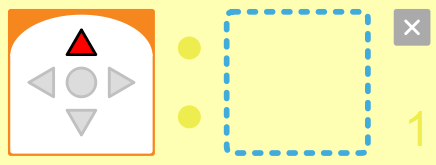
\includegraphics[width=.3\textwidth,keepaspectratio=true]{event-action-pair-yellow1}
&
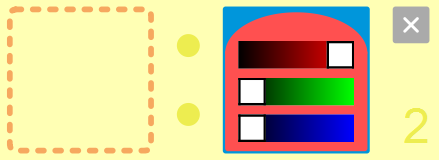
\includegraphics[width=.3\textwidth,keepaspectratio=true]{event-action-pair-yellow2}
\end{tabular}
\end{center}

Das linke goldfarbene Quadrat ist der Bereich für das Ereignis; das rechte blaue Quadrat ist der Bereich für die erste oder einzige Aktion. Das Paar mit dem gelben Hintergrund nennen wir das \emph{aktuelle} Paar.

\informationbox{Schnelle Eingabe}{Mittels Doppelklick kann man einen Ereignis- oder Aktionsblock direkt in den Programmierbereich übernehmen. Dabei wird er an der aktuellen Stelle positioniert (gelber Hintergrund).}


\informationbox{Die VPL Werkzeugleiste}{\cref{a.toolbar} umfasst eine Beschreibung aller Elemente der VPL Werkzeugleiste. Schauen Sie bei Gelegenheit nach bis Sie die Handhabung gelernt haben.}
